We examine two independent variables, traffic request pattern and pod
initialization time, with respect to the different scaling types' performance.
In other words, for reactive and predictive
auto-scaling, we examine the impacts of varying the request pattern of traffic
to our testing application and the impacts of differing pod initialization
times. This allows us to determine under what combinations of traffic request
patterns and pod initialization time predictive auto-scaling is most effective,
and also under what combinations it is the least effective. Furthermore, because
we utilize the same independent variables for all of the different scaling
types, and because these independent variables are relevant to all scaling
types, we can make comparisons across predictive and reactive auto-scaling.
For example, we could determine that predictive
auto-scaling outperforms reactive auto-scaling most
when pod initialization time is lengthy and the traffic pattern is a simple
linear slope, but predictive auto-scaling exhibits very little difference from
reactive auto-scaling when pod initialization time is very small and we see a
\textit{flash crowd} traffic pattern.

\subsection{Pod Initialization Time}

As will be discussed in detail in the later \textit{Tools} section, we've created a web
server application that allows us to specify any \textit{pod
initialization time} we desire. As such, we have considerable flexibility with
respect to what initialization time values we test. To begin, we decided to test the
following values: 5s and 135s.

We believe 5s and 135s are important independent variables to test because they
are indicative of different classes of applications that could be run on
Kubernetes. A pod initialization time of 5s is commonly found among web
application frameworks, as we showed when writing a simple HTTP server in Go and
using the Spring Java web application framework \cite{spring}. There web
frameworks initialized, and were ready to serve requests, in 1s and 5s
respectively. It is our strong belief that any web framework that simply
needs to initialize, without any external communicating our data, will
accomplish this task in under 5s. Thus, testing a pod initialization time of 5s
allows us to consider how any web application framework would perform with
predictive auto-scaling.

We derive a pod initialization time of 135s from a simulation of downloading a
shard database file, loading it into a database, and then starting a web
application to process data from said database. More specifically, our sample
pod downloaded a 25.2MB file and then batch inserted it into an Elasticsearch
database \cite{elasticsearch}. It then started a web application framework. In
all, this process took approximately 135s, although it is easy to imagine the
time varying based on the size of the initial shard file. The file we downloaded
came from an ElasticSearch tutorial on prepopulating a database
\cite{elasticsearch-import-some-data}, and thus we believe it is a fairly
representative size. By examining pod initialization times of 5s and 135s, we
are confident that we are capturing the majority of the potential use cases for
predictive auto-scaling.

We believe that there will be a \textit{sweet spot} of pod initialization times
for which predictive auto-scaling demonstrates the most benefits over reactive
auto-scaling. Obviously the smaller the pod intialization time value, the lesser
the difference between reactive and predictive auto-scaling, as predictive
auto-scaling predicts into the future a time closer and closer to the current
moment. However, the larger the pod initialization time value, the further into
the future we must predict the state of the application. While large pod
initialization times have the potential for considerable benefits when using
predictive auto-scaling, we can only realize that potential if predictions of
future application state are accurate. As the prediction window gets larger and
larger, accuracy becomes substantially more difficult to obtain.


\subsection{Traffic Request Pattern}

We are also interested in the impacts of different traffic patterns on scaling
performance. As such, we send our test web server application web requests in a
variety of patterns and examine which traffic pattern the scaling method handles
well, and which traffic pattern the scaling method does not handle well.
Moreover, we also examine scaling methods in relation to each other with respect
to different traffic patterns, seeking to answer for which traffic patterns
predictive auto-scaling is beneficial and which traffic patterns predictive
auto-scaling is detrimental or meaningless.

In this thesis we examine four different traffic patterns that we feel are
fairly indicative of the different traffic patterns a web application may face.
We entitle these patterns \textit{step-ladder}, \textit{jagged-edge},
\textit{increase-decrease}, and
\textit{flash-crowd}.\footnote{There are of course an infinite number of traffic
patterns that we could examine, and examining other options is an exciting
opportunity for future work.} We describe each of these patterns, and offer a
visual representation for each, below. Each pattern runs for at least twenty
minutes and at most forty minutes, and makes at most 20 requests per second.\footnote{All
traffic patterns have a start and end buffer at which they receive
only 1 request per second, to ensure we do not immediately overload the
application.} These values were chosen to give
space for the lengthier pod initialization times and to keep the network from
becoming too congested respectively. We can imagine the all traffic seen by a
typical web server as being composed of different combinations of these patterns
across longer time spans.

\begin{itemize}
  \item \textbf{step-ladder}: The traffic pattern \textit{step-ladder}, visible
    in Figure \ref{fig:step-ladder}, represents a web server which faces a load
    pattern which increases immediately at predicted intervals. This scenario
    can be seen as representing, for example, an video streaming website which
    experiences predictible increases in traffic as different shows are
    streamed. This traffic pattern begins with 1 request per second for 3
    minutes, before immediately increasing to 4 requests per second. The process
    of increasing by 3 requests per second and then staying constant for 3
    minutes continues for 6 more iterations until it reaches 19 requests per
    second.

    \begin{figure}[!h]
      \centerline{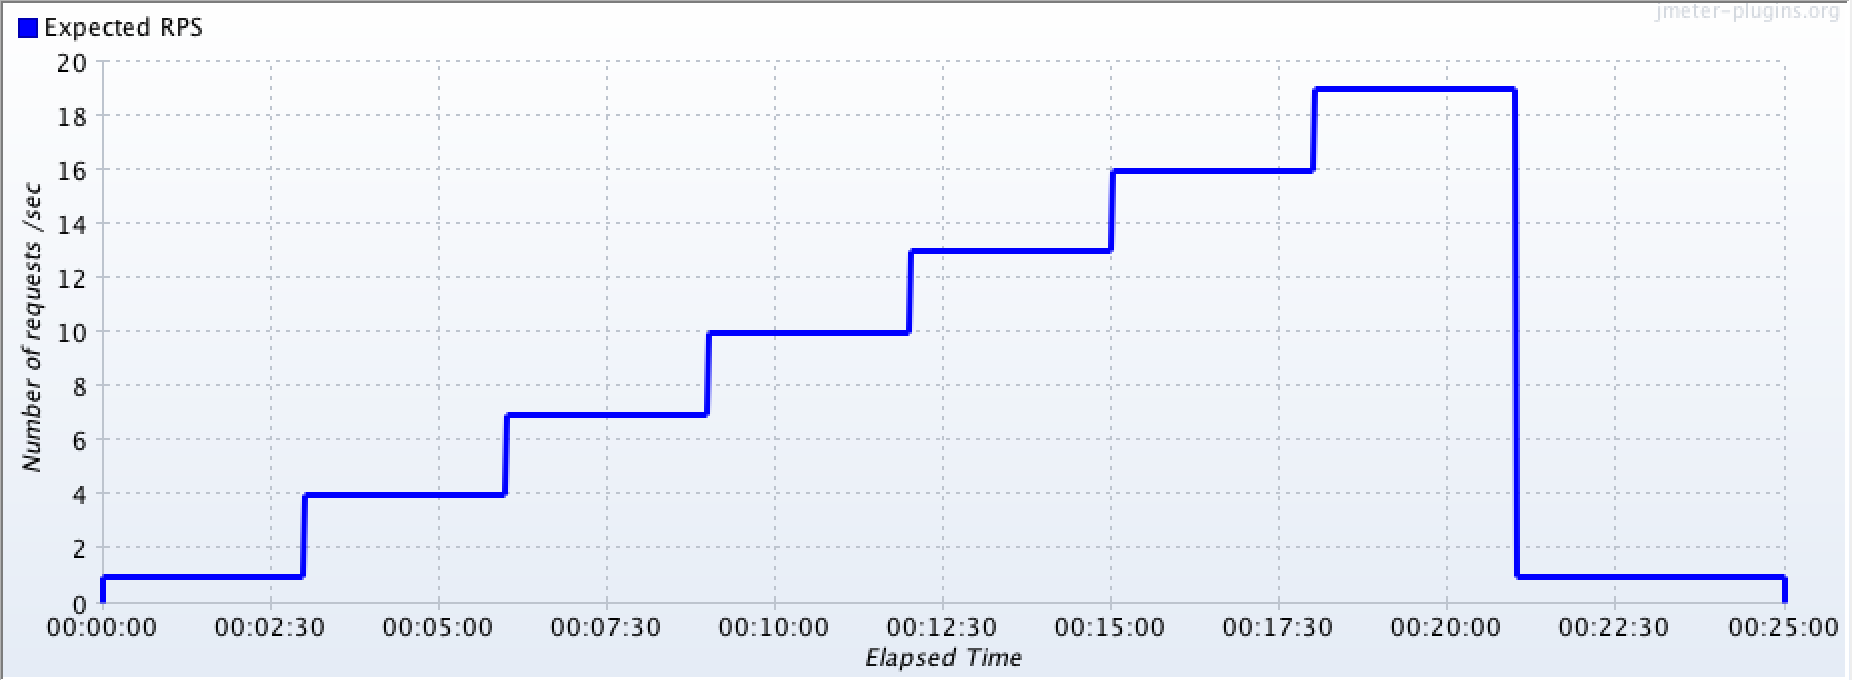
\includegraphics[scale=.4]{step-ladder.jpg}}
      \caption{The step-ladder Traffic Pattern}
      \label{fig:step-ladder}
    \end{figure}

  \item \textbf{jagged-edge}: The traffic pattern \textit{jagged-edge}, visible
    in Figure \ref{fig:jagged-edge}, is similar to \textit{step-ladder},
    although it reflects a more gradual increase and decrease in load. Thus, it
    applies to a similar scenario as \textit{step-ladder}. It begins at 1
    request per second before 3 minutes before increasing to 10 requests per
    minute over the course of 5 minutes. It then decreases to 5 requests per
    second over the course of 2 minutes. This pattern of increasing by 10
    requests per second over the course of 5 minutes and then decreasing by 5
    requests per second over the course of 2 minutes continues until reaching 20
    requests per second, and which point we transition to the end buffer period
    of 1 request per second for 5 minutes.

    \begin{figure}[!h]
      \centerline{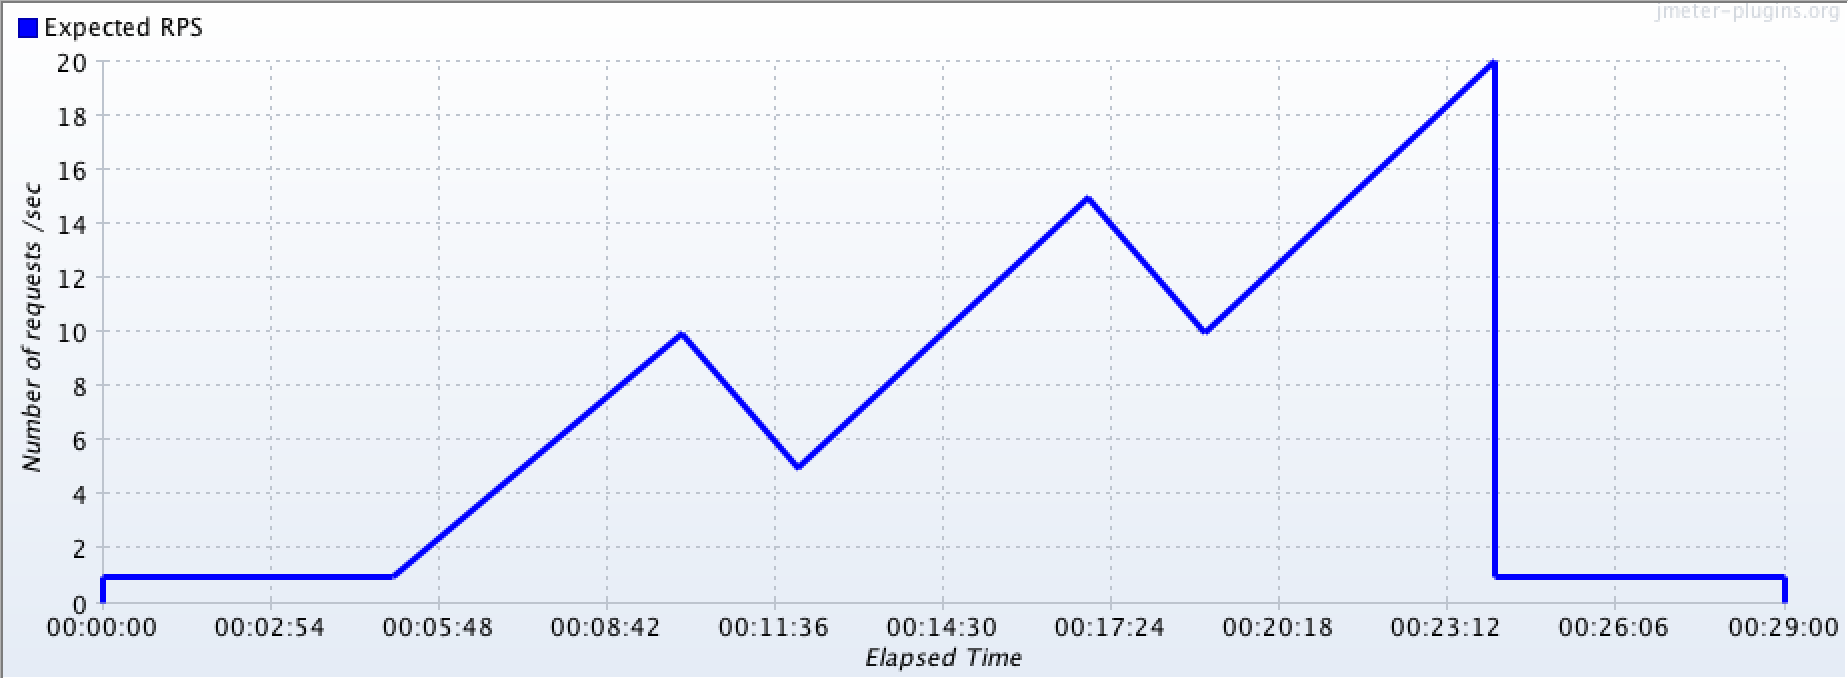
\includegraphics[scale=.4]{jagged-edge.jpg}}
      \caption{The jagged-edge Traffic Pattern}
      \label{fig:jagged-edge}
    \end{figure}

  \item \textbf{increase-decrease}: The traffic pattern
    \textit{increase-decrease}, visible in Figure \ref{fig:increase-decrease},
    represents a web server facing constantly increasing and then constantly
    decreasing load. This scenario can be seen as representing, for example, a
    restaurant in which people increasingly visit the site as it becomes closer
    and closer to a meal time, and decreasingly visit the site as a meal time
    becomes farther and farther away. After five minutes of initialization at
    1 request per second, our load
    generator builds from sending 1 request per second to 20 requests per
    second over the course of 15 minutes. After reaching the apex, the traffic
    generator then reduces from sending 30 requests per seconds to sending 1
    request per second, again over the course of 15 minutes.

    \begin{figure}[!h]
      \centerline{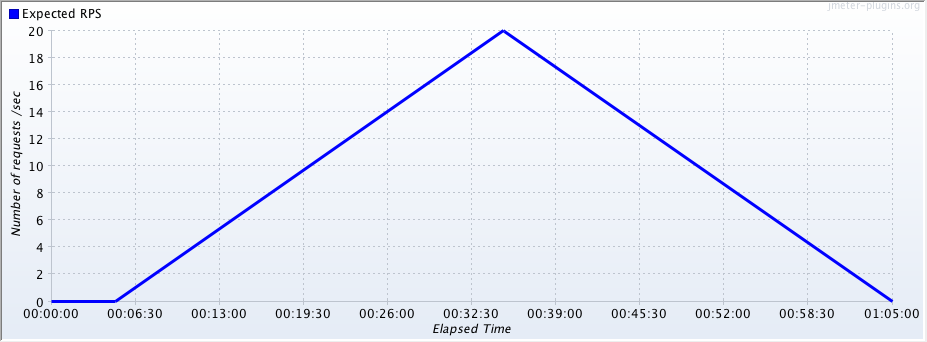
\includegraphics[scale=.4]{increase-decrease.jpg}}
      \caption{The increase-decrease Traffic Pattern}
      \label{fig:increase-decrease}
    \end{figure}

  \item \textbf{flash-crowd}: The traffic pattern \textit{flash-crowd}, visible
    in Figure \ref{fig:flash-crowd}, represents a web server facing a suddenly
    increasing, and then suddenly decreasing, amount of load. This scenario is
    indicative of, for example, a news website which will suddenly receive a
    short-lived burst of traffic when a major story hits. After five minutes of
    sending 1 request per second, our load generator
    builds from sending 1 request per second
    to sending 5 requests per second, over the course of 5 minutes. Then, in
    just 2 minutes, our load generator jumps from sending 5 requests per second
    to sending 20 requests per second. After reaching the apex, the traffic
    generator decreases from sending 20 requests per second to sending 5
    requests per second, again in just 2 minutes. Finally, our load generator
    decreases from sending 5 requests per second to 1 request per second, over
    the course of 5 minutes, before transitioning to the end buffer period of 1
    request per second for 5 minutes.

    %% We use flash-crowd-short although we refer to it as flash-crowd.
    \begin{figure}[!h]
      \centerline{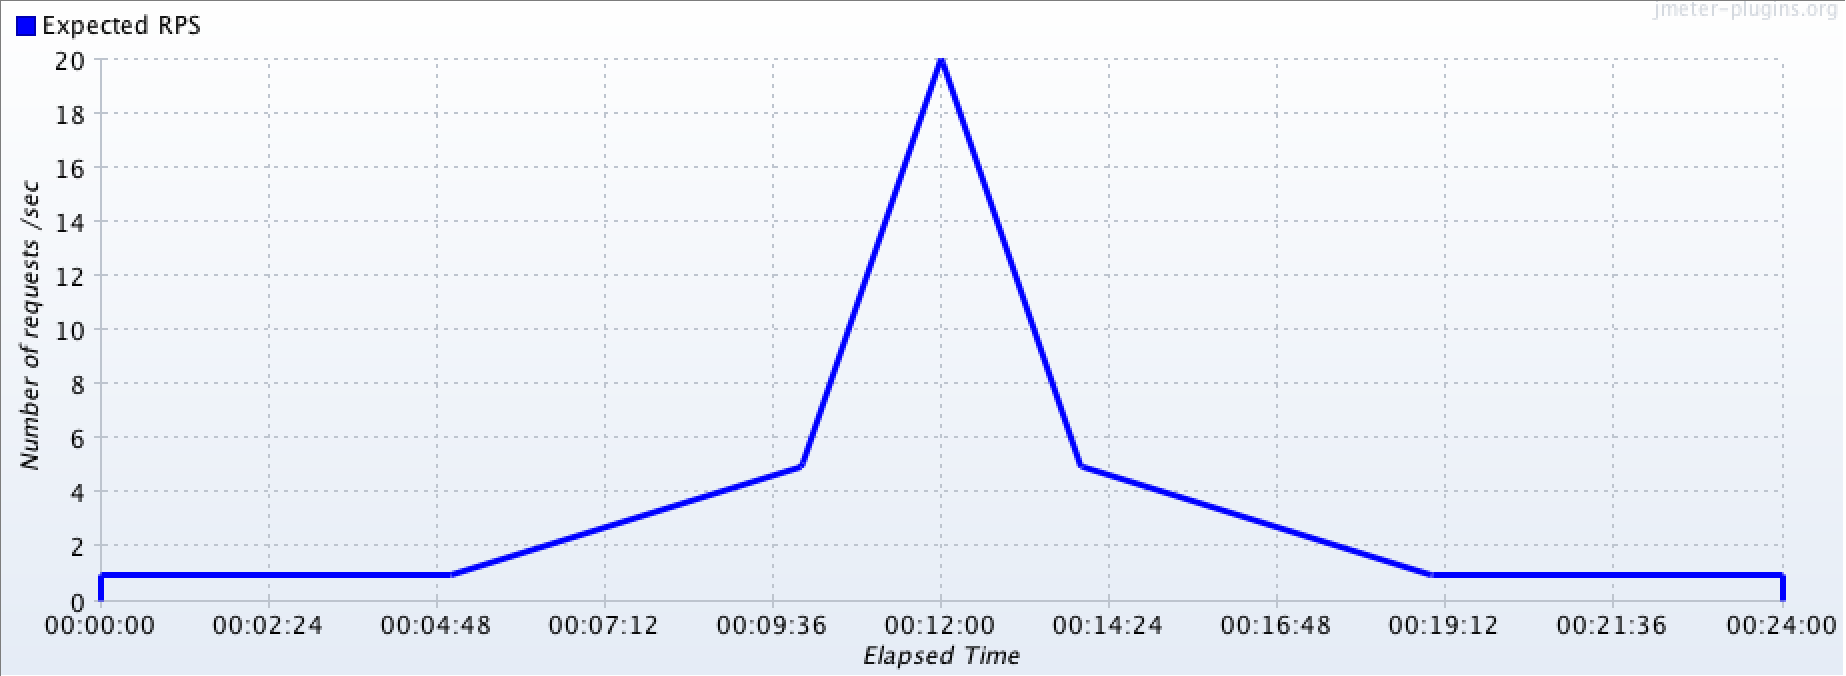
\includegraphics[scale=.4]{flash-crowd-short.jpg}}
      \caption{The flash-crowd Traffic Pattern}
      \label{fig:flash-crowd}
    \end{figure}

\end{itemize}

